\chapter{REVIEW OF RELATED LITERATURE}
{\baselineskip=2\baselineskip
This review centers on studies and technologies that have contributed valuable insights to the design and development of this research, specifically in the area of multi-camera tracking systems and customer behavior analysis. It examines various advancements in multi-camera systems, object detection techniques, and their practical applications to understand customer behaviors in retail environments.
%-----------------------------------------------------------------------------------------------------------------------
\section{Intelligent Marketing}
Customer behavior analysis is crucial in intelligent marketing, offering valuable insights into how customers interact with products and navigate store environments. Several studies highlight the significance of product placement, store layout, and time spent in different zones on purchasing decisions. For example, \cite{Kim2019} found that time spent in specific store areas significantly impacted sales more than overall stay time, suggesting that strategic product placement can directly drive revenue. Similarly, other research emphasizes how rearranging visual merchandising displays can alter customer movement patterns and improve sales in targeted store zones.

Traditionally, customer behaviors were analyzed through surveys, manual observations, and customer feedback. While these methods provided valuable insights, they were limited in scale, real-time data capture, and accuracy. These approaches often relied on subjective interpretation, making gathering large-scale, precise data challenging. However, the advent of new technologies, such as video analytics and IoT sensors, has revolutionized the field of customer behavior analysis. \cite{Erlina2023} demonstrate how the YOLO algorithm facilitates real-time visitor detection and movement tracking, allowing businesses to classify and monitor customer behavior. Likewise, \cite{Kim2019} show that IoT devices can track customer locations and generate data on movement patterns, enabling a more comprehensive and accurate analysis of customer behaviors.

Computer vision and object detection technologies are central to customer tracking and footfall analysis. \cite{Cobos2019} underscore the utility of multiple-object tracking systems in analyzing customer movement and traffic flow through video feeds. AI-based systems, such as those explored by \cite{Cabahug2023}, take this further by automating customer counting and mapping in intelligent retail environments. These vision-based technologies provide real-time data, allowing businesses to gather insights into store performance and optimize operations based on precise customer behavior.

Heat map generation is a notable tool in this field, as it visually represents customer dwell times and movement patterns. Heat maps are an increasingly popular method for identifying high-traffic areas in retail spaces. \cite{Cabahug2023} discuss how motion heat maps can highlight zones with high foot traffic, aiding in decisions about store layout optimization. This technique is effective for customer tracking and enhances store performance analysis, allowing retailers to understand how the layout impacts consumer behavior and adjust marketing strategies accordingly.

Integrating computer vision, IoT, and AI-based technologies in retail settings reshapes how businesses analyze and respond to customer behaviors. These innovations provide more accurate, large-scale, real-time data, supporting more informed marketing and store management decision-making.

\section{Technological Frameworks and Systems for Retail Analysis}
As the retail landscape grows increasingly competitive, businesses are turning to advanced technological frameworks to gather insights into customer behaviors and store performance. These systems utilize a combination of AI, machine learning, and IoT technologies to track and analyze customer behavior, enhancing marketing and operational strategies. This section provides an overview of existing retail analytics systems and the adaptation of surveillance technologies for business insights. It also compares system architectures used in multi-camera setups for retail analytics.

Retail analytics systems have evolved from traditional point-of-sale (POS) data analysis to more sophisticated methods incorporating computer vision, multi-camera tracking, and AI algorithms. These modern systems offer a comprehensive view of customer interactions and behaviors in real-time, providing valuable data on foot traffic, dwell times, and purchasing behaviors. For instance, systems like those presented by \cite{Cabahug2023} employ AI-based customer counting and foot traffic tracking, which aids in assessing store performance and guiding decisions on product placement and layout optimization.

Similarly, technologies like YOLO, used in visitor detection systems  \citep{Erlina2023},  apply object detection algorithms to categorize customers and track their movements throughout the store. These systems generate insights beyond simple visitor numbers, offering detailed data on customer behaviors. This enables small and large retailers to optimize their operations based on real-time tracking data, ultimately improving their ability to respond to customer behavior.

Surveillance technologies, which were initially developed for security purposes, have found new applications in retail analytics. Closed-circuit television (CCTV) cameras, once primarily used for loss prevention, are now critical for customer behavior analysis. \cite{Cobos2019} describe a system that leverages CCTV footage and multi-object detection algorithms to track customers and analyze traffic flow within retail stores. By adapting these technologies for business insights, retailers can evaluate the effectiveness of marketing campaigns, refine store layouts, and track customer engagement in specific areas.

\cite{Xie2024} further illustrate the adaptation of multi-camera systems, initially designed for crowd management and surveillance, to retail settings. These systems track customers across camera views using advanced features like geometric consistency and Re-ID correction mechanisms. This approach ensures accurate tracking even in environments with high levels of occlusion or varying camera angles, providing reliable data for marketing and customer behavior analysis.

Regarding system architecture, retail analytics platforms can generally be categorized into cloud-based and edge-based systems. Cloud-based architectures transmit video data or analytics information to centralized cloud servers for processing and storage. These highly scalable systems make them well-suited for large retail chains with multiple locations. Cloud-based solutions benefit from powerful computational resources and advanced machine-learning models that enable predictive analytics. However, they may face latency issues due to the need to transfer large amounts of data to remote servers, which can hinder real-time analysis.

\cite{Kulkarni2023} discuss the advantages of cloud-based systems in enhancing retail operations through AI and computer vision. They note, however, that maintaining real-time performance and ensuring data security can be challenging when relying heavily on cloud servers.

On the other hand, edge computing offers an alternative architecture by processing data closer to its source, typically on local devices such as in-store servers or cameras. This reduces latency and enables real-time analytics, making it ideal for high-speed customer tracking and immediate decision-making. For example, systems like those proposed by \cite{Erlina2023}, which use single-board computers for visitor detection, demonstrate the trend toward edge-based retail systems. These solutions offer faster processing times and lower bandwidth requirements, allowing retailers to conduct complex analytics without depending on external cloud servers.

While edge computing is particularly advantageous for smaller retailers who may lack the resources to implement large-scale cloud solutions, it does have limitations in terms of scalability and computational power compared to cloud-based systems. Despite this, the shift toward edge-based systems reflects the need for real-time analytics and localized decision-making in an increasingly data-driven retail environment.

\section{Object Detection and Multi-Camera Systems}
Object detection has evolved significantly, transitioning from traditional methods to advanced AI-powered algorithms that provide real-time tracking and insights across retail, surveillance, and autonomous driving industries. This section explores the development of object detection technologies, modern techniques, challenges, and the role of multi-camera systems in enhancing detection accuracy.

Early object detection methods heavily relied on handcrafted features and simple classifiers. For instance, Haar cascades were used for face detection, offering basic results. More advanced techniques like the Scale-Invariant Feature Transform (SIFT) and Histogram of Oriented Gradients (HOG) improved detection accuracy by capturing more detailed image features. However, these methods struggled with complex scenes, variable lighting conditions, and occlusions. The advent of deep learning marked a turning point, allowing models to automatically extract hierarchical features from raw image data, significantly improving detection performance in challenging environments.

Recent advances in deep learning have led to the development of several state-of-the-art object detection algorithms, each with distinct strengths and limitations. YOLO is renowned for its real-time detection capability. It uses a single neural network to directly predict bounding boxes and class probabilities from full images in one evaluation. It is ideal for applications like retail monitoring, where speed is critical \citep{Erlina2023}. However, YOLO trades off some accuracy compared to other techniques, particularly when detecting smaller objects.

In contrast, Faster R-CNN is a two-stage detector that generates region proposals before classifying these regions into objects. This highly accurate approach suits applications requiring detailed analysis, such as surveillance and precision-focused retail environments \citep{Chen2022}. However, Faster R-CNN is slower than YOLO, which limits its use in real-time scenarios.

Another prominent algorithm is SSD (Single Shot Multibox Detector), which balances speed and accuracy. Like YOLO, SSD performs object detection in a single pass but improves accuracy using multiple feature maps of varying resolutions. This approach is ideal for detecting objects of different sizes, making SSD a versatile option for applications that require a balance between real-time performance and precision.

Despite these advancements, object detection faces several challenges in real-world environments. Occlusions, where objects are partially or fully hidden, pose a significant challenge, especially in crowded retail spaces. Single-camera systems, in particular, struggle with occlusions due to their limited perspectives. Additionally, varying lighting conditions, such as shadows or glare, can significantly reduce detection accuracy, even for the most advanced models. Poor illumination further complicates detection in low-light environments, while cluttered scenes add noise that models must differentiate from target objects.

Although cost-effective and easier to deploy, single-camera systems come with inherent limitations. Their lack of depth perception and vulnerability to occlusion and blind spots restricts their ability to capture dynamic environments fully. In contrast, multi-camera systems offer a broader, more comprehensive view by covering the same scene from multiple angles. This setup enables more accurate tracking of objects, even in cases of occlusion. As \cite{Xie2024} demonstrated, multi-camera systems can leverage geometric consistency and state-aware Re-ID correction to maintain accurate tracking in retail stores, where customers often move between camera views.

Synchronization and calibration are essential to ensuring the effectiveness of multi-camera systems. Synchronization ensures that frames captured at the exact moment from different cameras are analyzed together, allowing for seamless tracking across multiple views. Calibration aligns the cameras in a standard coordinate system, ensuring accurate mapping of object locations across different perspectives. Techniques such as geometric consistency, discussed by \cite{Li2023}, help maintain tracking accuracy across cameras by aligning spatial and temporal data.

Multi-camera systems have been widely adopted across various domains. In surveillance, they monitor large areas, providing comprehensive coverage and enabling tracking across multiple zones \citep{Xie2024}. In autonomous driving, multi-camera systems detect and track objects, such as pedestrians and other vehicles, from various angles to enhance safety and navigation. Retail environments also adopt multi-camera setups to monitor customer behaviors, track foot traffic, and analyze dwell times in high-traffic areas \citep{Cabahug2023}. This allows retailers to optimize store layouts and enhance customer experiences.

An essential aspect of multi-camera systems is data fusion, where information from multiple camera feeds is aggregated to create a cohesive view of the scene. Data fusion mitigates challenges like occlusion, enhancing overall object detection accuracy. \cite{Xu2021} explored multi-view feature fusion for person Re-identification, showing that combining data from different angles provides a more complete representation of objects, improving tracking effectiveness.

The evolution of object detection has been transformative, with modern deep learning algorithms overcoming many limitations of traditional methods. Multi-camera systems enhance detection accuracy by providing a more comprehensive view of dynamic environments, addressing occlusion and lighting variability. These advancements have broad applications in retail and autonomous driving industries, showcasing the growing importance of AI-powered object detection technologies.

\subsection{Multi-Camera Object Detection in Retail Applications}
Multi-camera object detection has been successfully applied in various retail case studies, showcasing its potential to enhance store performance and customer experience. For instance, \cite{Cabahug2023} developed a computer vision system to track and count customers across different zones of a retail store. Their system utilized heat maps to identify high-traffic areas, which enabled them to suggest layout optimizations to improve overall store performance. Similarly, \cite{Cobos2019} employed multi-camera systems to monitor customer and shopping cart movements, providing retailers valuable insights into traffic flow and customer behavior patterns.

Recent studies have further demonstrated the power of computer vision for in-store behavioral analysis. One example is a study by \cite{Shili2024} on advanced customer behavior tracking and heatmap analysis using YOLOv5 and DeepSORT. This approach leveraged object detection and tracking to analyze real-time video footage of customer movements within retail spaces. The system generated heat maps that visualized movement patterns and zone engagement, offering actionable insights into customer preferences and product popularity. This data allows retailers to choose product placements, optimise store layout, and target marketing strategies. The framework was also noted for its scalability and minimal intervention requirements, making it a practical solution across various retail environments. This study highlights the growing importance of computer vision technologies in enabling data-driven retail decision-making and personalized customer experiences.

Despite its benefits, object detection in retail environments presents unique challenges. One major issue is occlusion, where shelves, other customers, or merchandise obstruct the camera’s view, making it difficult to detect and track individuals accurately. Another challenge is variable lighting within retail stores, as inconsistent lighting conditions, ranging from brightly lit areas to dim corners, can affect the accuracy of object detection models. Furthermore, large crowds can cause misidentifications or tracking errors, particularly in busy stores or during peak shopping hours when the density of customers increases.

Multi-camera systems offer several advantages to address these challenges. Firstly, they enable comprehensive tracking by covering blind spots and occluded areas, ensuring customers are accurately tracked throughout the store. Secondly, multi-camera setups provide enhanced insights by capturing customer movements from various angles, allowing retailers to generate heat maps that reveal high-traffic areas, dwell times, and movement patterns. These insights support more effective decisions on store layouts and product placements. Finally, multi-camera systems improve accuracy by reducing the likelihood of missed detections, especially in environments with heavy occlusions or inconsistent lighting conditions.

Benchmark datasets and evaluation protocols have been introduced to support the development and evaluation of such systems. One notable example is MMPTRACK, a large-scale benchmark for multi-camera multiple object tracking (MC-MOT) \citep{Han2023}. This dataset focuses on person tracking across numerous overlapping and non-overlapping camera views, specifically in complex environments such as airports, subway stations, and malls. MMPTRACK includes various evaluation metrics like MOTA, IDF1, and others, which allow researchers and developers to assess the accuracy and robustness of multi-camera tracking systems under real-world conditions. Similarly, the study by \cite{Fei2023} reviewed a range of performance metrics for multi-object, multi-camera tracking systems in intelligent transportation. Although applied to traffic settings, the evaluation metrics outlined, such as MOTA, IDF1, false positives, and false negatives, are broadly applicable and were adopted in this study to evaluate the SUBAY system. Integrating insights from such benchmarks enables systems like SUBAY to adopt state-of-the-art evaluation practices and validate their effectiveness in live retail deployments.

\subsection{Deep Learning and Artificial Intelligence in Retail}
Artificial intelligence (AI), particularly deep learning, has become integral to object detection in retail environments. Advanced algorithms like YOLO and Faster R-CNN are commonly employed to detect and track customers in real time, providing valuable insights into their behaviors. These models can be trained on extensive datasets, enhancing detection accuracy even in complex settings such as crowded or visually cluttered stores.

Residual neural networks, such as ResNet (Residual Network), are foundational to the performance of many deep learning-based detection and tracking models. ResNet addresses the degradation problem in deep networks by allowing layers to learn residual mappings with shortcut connections \citep{GeeksforGeeks2025}. These skip connections train deeper networks without suffering from vanishing gradients, significantly improving feature extraction capabilities. This is particularly useful in high-variance environments like retail stores.

Building upon these architectural advancements, models like Omni-Scale Network (OSNet) have been designed explicitly for person Re-identification (Re-ID) tasks. OSNet captures features at multiple spatial scales simultaneously, allowing it to discern subtle appearance differences across camera views \citep{Boujou2022}. This is particularly valuable in multi-camera retail setups where customer appearances vary due to angles, lighting, or occlusion. By learning omni-scale features, OSNet supports more robust customer tracking across zones, helping to maintain persistent identification without confusion between individuals.

Among the many object detection algorithms developed for real-time applications, the YOLO family of models has gained widespread recognition in computer vision. YOLO models are designed for high-speed, high-accuracy detection tasks, especially for time-sensitive retail scenarios. The series has evolved from YOLOv1 to YOLOv10, with each iteration introducing improvements in detection accuracy, computational efficiency, and architectural innovations. For example, YOLOv5 focused on lightweight deployment and ease of use, while YOLOv7 and YOLOv8 further refined detection speed and model precision. YOLOv9 introduced the effective use of transformer-based modules for long-range spatial reasoning, but it is YOLOv10 that currently stands out for its balance of performance and real-time readiness.

YOLOv10, the latest in the series as of this study’s implementation, outperforms previous versions across key benchmarks, including mean Average Precision (mAP), inference speed (frames per second), and computational efficiency (GFLOPs). Its architecture incorporates innovations such as RT-DETR (Real-Time Detection Transformer) and features optimized for edge devices and high-performance computing environments, making it highly adaptable to real-world retail deployments. These enhancements allowed the system to accurately detect multiple customer instances in crowded scenes while maintaining a consistent frame rate necessary for live CCTV integration.

YOLOv10 consistently ranks among the top-performing models in accuracy and speed, making it the most suitable model for the SUBAY system’s retail environment. Its performance advantages and its ability to be fine-tuned on domain-specific footage make it an ideal choice for customer detection in dynamic in-store conditions.

Beyond real-time detection, AI plays a pivotal role in predicting customer behaviors. By analyzing past shopping data and current movement patterns, predictive models can forecast customer behavior, such as potential purchases, preferred navigation paths, or areas of interest within the store. This allows retailers to personalize shopping experiences, tailor product recommendations, and adjust marketing strategies accordingly \citep{Kulkarni2023}. For example, data-driven insights into customer traffic patterns inform decisions on where to place promotions or how to redesign store layouts for maximum engagement.

However, using AI to track and predict customer behaviors raises significant privacy concerns. As retailers gather increasingly detailed information on customer behavior, ethical considerations around data security and privacy come to the forefront. Ensuring that data is anonymized and customer identities are protected is crucial to addressing these concerns. Many systems now require explicit customer consent before tracking begins, while sophisticated anonymization techniques are applied to video feeds to mitigate privacy risks. Furthermore, regulatory frameworks such as the General Data Protection Regulation (GDPR) are essential in safeguarding customer data, ensuring that businesses handle it responsibly and transparently.

While AI has greatly enhanced object detection and predictive analytics in retail, its use comes with critical ethical considerations, particularly concerning privacy. Addressing these challenges through robust data protection measures and regulatory compliance is essential for maintaining consumer trust and ensuring the responsible deployment of AI technologies in retail settings.

\section{Synthesis Matrix}
The reviewed literature highlights several gaps in current research on multi-camera systems in retail. Firstly, while multi-camera systems are widely discussed in areas like surveillance and autonomous driving, their optimization for retail environments remains under-explored. Specifically, existing studies do not address challenges such as occlusion from shelves and variable lighting conditions. Secondly, there is a lack of research focusing on real-time data fusion techniques that integrate multiple camera feeds to enhance object detection accuracy in retail settings. Additionally, while AI-based object detection models are becoming increasingly prevalent, there is a notable gap in integrating these models with behavior prediction frameworks tailored to retail. Further research is needed to develop AI models that predict customer actions in real-time, which could significantly improve customer engagement and optimize store layouts.

Moreover, the literature inadequately addresses privacy concerns related to real-time multi-camera systems, particularly the anonymization techniques required to comply with regulations like the GDPR, leaving another important area for future investigation.

Despite these gaps, implementing multi-camera object detection systems optimized for retail holds significant potential. Such systems can provide comprehensive customer tracking, reducing occlusions and blind spots while delivering valuable insights into customer paths, dwell times, and product interactions. These insights will enable retailers to optimize store layouts and product placements, ultimately enhancing the shopping experience and sales outcomes. Furthermore, by integrating multi-camera systems with AI-driven behavior prediction models, retailers can forecast customer movements and likely purchases in real-time, leading to more personalized customer engagements and targeted marketing strategies.

Advanced data fusion techniques can further refine the accuracy of heat maps and traffic patterns, offering actionable insights into store performance, identifying bottlenecks, and highlighting high-traffic areas. However, retailers must address the growing privacy concerns by adopting real-time anonymization techniques in multi-camera systems to leverage these advancements. This would allow businesses to maintain customer trust and ensure regulatory compliance while extracting valuable data for retail analytics. By addressing these gaps, future research can drive the development of more sophisticated retail analytics tools, transforming customer tracking and behavior analysis.

Table~\ref{tab:related-studies} below summarizes key findings from the reviewed literature and highlights gaps this study aims to fill. It also organizes findings based on each study’s methodologies, technology or algorithm used, findings, and relevance to this study.

Based on the synthesis of the ten studies from the matrix as shown in Table~\ref{tab:related-studies}, several advancements in computer vision models, object detection, and multi-camera tracking systems \citep{Xie2024,Amosa2023} have been evaluated and incorporated into the design of the current conceptual framework. Many of these studies emphasized the effectiveness of algorithms such as YOLO  \citep{Chen2022,Erlina2023} and DeepSORT (Simple Online and Realtime Tracking with a Deep Association Metric) \citep{Li2023} for detecting and tracking multiple individuals in crowded environments.

\begin{landscape}  % Begin landscape mode
	% Add custom page break control
	\setlength{\LTpre}{0pt}      % Remove space before longtable
	\setlength{\LTpost}{0pt}     % Remove space after longtable
	
	% Define maximum rows per page for better control
	% Adjust this number based on your needs
	\newcounter{rowcount}
	\setcounter{rowcount}{0}
	
	\begin{longtable}{|p{2.5cm}|p{2.5cm}|p{2.7cm}|p{2.7cm}|p{2.5cm}|p{2.5cm}|p{2.5cm}|}  % Adjusted column widths
		\caption[Synthesis Matrix]{\newline \newline Synthesis Matrix} \label{tab:related-studies} \\
		
		\hline 
		\textbf{Study Title} & \textbf{Author(s) and Year} & \textbf{Methodology} & \textbf{Technology or Algorithm Used} & \textbf{Findings/ Results} & \textbf{Relevance to Current Study} & \textbf{Limitations} \\ 
		\hline 
		\endfirsthead
		
		\multicolumn{7}{l}{{\tablename\ \thetable{} -- \textit{continued from previous page}}} \\
		\hline
		\textbf{Study Title} & \textbf{Author(s) and Year} & \textbf{Methodology} & \textbf{Technology or Algorithm Used} & \textbf{Findings/ Results} & \textbf{Relevance to Current Study} & \textbf{Limitations} \\ 
		\hline 
		\endhead
		
		\hline 
		\multicolumn{7}{|r|}{{Continued on next page}} \\ 
		\hline
		\endfoot
		
		\hline
		\endlastfoot
		
		% Page 1 - First 7 rows similar to your Google Docs layout
		% Row 1
		Multi-camera multi-object tracking: A review of current trends and future advances
		& Amosa, Temitope Ibrahim; Sebastian, Patrick; Izhar, Lila Iznita; Ibrahim, Oladimeji; Ayinla, Lukman Shehu; Bahashwan, Abdulrahman Abdullah; Bala, Abubakar; Samaila, Yau Alhaji (2023)
		& Literature review of trends and advancements in multi-camera tracking technologies.
		& Various MCT algorithms were reviewed, including data association and occlusion handling.
		& Summarized outcomes of 30 MCT algorithms and identified promising future directions.
		& Provides insights into MCT advancements relevant to improving retail analytics.
		& This study provides a theoretical review of MCT algorithms but lacks practical, implementa-\newline tion-based validation in real-world retail environments.\\
		\hline
		
		% Row 2
		Customer Counting and Mapping for Intelligent Retail Environment using Computer Vision
		& Cabahug, Jhon Lloyd; Gulle, Anferny Glenn; Macarayo, Dave; Perez, Leander Danilo (2023)
		& Computer vision techniques for customer counting and tracking in retail environments.
		& Computer vision techniques, motion heat maps
		& Achieved an F1 score of 95.78\%, effectively visualizing foot traffic, and challenges in congested areas.
		& Demonstrates potential for using computer vision in retail, though with limitations in crowded areas.
		& The system struggles to maintain high accuracy in crowded and congested areas with multiple customer overlaps. \\
		\hline
		
		% Row 3
		Research on Pedestrian Detection and DeepSORT Tracking in Front of an Intelligent Vehicle Based on Deep Learning
		& Chen, Xuewen; Jia, Yuanpeng; Tong, Xiaoqi; Li, Zirou (2022)
		& Pedestrian detection and tracking using an improved YOLO model and DeepSORT algorithm for intelligent vehicle applications.
		& YOLO detection model, DeepSORT, Kalman filter
		& Enhanced detection of small and partially blocked pedestrians reduced false detection rates.
		& The improvements made in YOLO could be adapted to improve customer detection in retail environments.
		& Although effective in vehicle contexts, the model is not specifically optimized for indoor retail scenarios with complex layouts and varying lighting. \\
		\hline
		
		% Row 4
		Retail Traffic-Flow Analysis Using a Fast Multi-Object Detection and Tracking System
		& Cobos, Richard; Hernandez, Jefferson; Abad, Andres G. (2019)
		& A multiple-object tracking system was applied to retail traffic flow analysis.
		& Tracking-by-detection paradigm, an ensemble of detectors, heat maps
		& Successfully generated traffic-flow heat maps, reducing hardware costs through CCTV camera systems.
		& This paper highlights the use of heat maps to analyze customer movement, which is relevant to understanding footfall and behaviors in retail.
		& The focus is limited to traffic flow patterns and does not explore customer behavior or interaction within product zones. \\
		\hline
		
		% Row 5
		A YOLO Algorithm-based Visitor Detection System for Small Retail Stores using Single Board Computer
		& Erlina, Tati and Fikri, Muhammad (2023)
		& YOLO-based visitor detection system utilizes a single onboard computer to monitor small retail store visitors.
		& YOLOv4-tiny algorithm
		& Achieved mAP of 89.21\%, enabling small business owners to track visitors and optimize operations.
		& Demonstrates using YOLO in small-scale retail, indicating its scalability for larger retail environments.
		& The single-camera system lacks scalability and may not maintain accuracy in larger or more dynamic store environments. \\
		\hline
		
		% Row 6 - Match the exact layout from screenshot where page 1 ends with 7 rows
		Multi-Object Multi-Camera Tracking Based on Deep Learning for Intelligent Transportation: A Review
		& Fei, Lunlin, and Han, Bing (2023)
		& Review of MOMCT systems with a focus on deep learning.
		& Deep learning-based detection and tracking, evaluation through visualization, benchmarking
		& Analyzed object detectors, datasets, metrics, and identified future challenges for MOMCT.
		& Provides foundational insight on applying deep learning and MOMCT to other domains such as retail environments.
		& The review is focused on transportation systems and does not address challenges specific to indoor retail tracking applications. \\
		\hline
		
		% Row 7
		MMPTRACK: Large-scale Densely Annotated Multi-camera Multiple People Tracking Benchmark
		& Han, Xiaotian; You, Quanzeng; Wang, Chunyu; Zhang, Zhizheng; Chu, Peng; Hu, Houdong; Wang, Jiang; Liu, Zicheng (2023)
		& Creation of a large-scale dataset using auto-annotation and 3D tracking.
		& 3D tracking using overlapped and calibrated depth + RGB cameras, manual refinement of auto-generated labels
		& The researchers created a densely labeled multi-camera tracking dataset and tested it using two multi-camera trackers and a ReID model across five environments.
		& This provides a benchmark dataset supporting the reliable evaluation of multi-camera trackers in cluttered environments. It shows the potential of 3D-enhanced multi-camera systems in solving occlusion, which is valuable for indoor customer tracking.
		& Densely annotated 3D data makes the system resource-intensive and impractical for lightweight deployment. \\
		\hline
		
		% Force page break after the first 7 rows to match screenshot layout
		\pagebreak
		
		% Page 2 - Continue with remaining rows
		% Row 8
		Location-Based Tracking Data and Customer Movement Pattern Analysis for Sustainable Fashion Business
		& Kim, Jonghyuk; Hwangbo, Hyunwoo; Kim, Sung Jun; Kim, Soyean (2019)
		& Indoor positioning and wireless sensors track customer movement patterns in a fashion retail store.
		& Indoor positioning, wireless sensor devices, and fingerprinting techniques
		& The stay time in specific zones impacted sales more than the total stay time in the store.
		& Highlights the importance of customer movement analysis for retail performance, applicable for multi-camera tracking.
		& The reliance on wireless sensors limits the depth of behavioral tracking and lacks visual confirmation of customer actions. \\
		\hline
		
		% Row 9
		Utilizing Gen AI and Computer Vision for Applications in the Retail Sector
		& Kulkarni, Nilesh D. and Bansal, Saurav (2023)
		& Analyse AI and computer vision applications in retail, including inventory management and store layout optimization.
		& AI, Computer Vision, Gen AI
		& Demonstrated AI's potential in revolutionizing retail through store layout optimization and personalized experiences.
		& Highlights the necessity of AI adoption in retail for advanced tracking and customer behavior analysis.
		& The study is largely conceptual and does not demonstrate actual deployment or testing of AI-based tracking systems.\\
		\hline
		
		% Row 10
		Cross-Camera Multi-Object Tracking based on Person Re-Identification and Spatial-Temporal Constraints.
		& Li, Jiayue and YanPiao, N. (2023)
		& Cross-camera multi-target tracking using spatial-temporal constraints to improve accuracy and reduce occlusion effects.
		& Spatial-temporal probability model, person Re-ID
		& Improved person trajectory correlation across cameras, effective in reducing occlusion influences.
		& Provides valuable strategies for dealing with occlusion and accuracy in multi-camera retail tracking.
		& While effective in improving accuracy, the system's complexity and lack of web-based accessibility limit its usability in retail settings.\\
		\hline
		
		% Row 11
		Advanced Customer Behavior Tracking and Heatmap Analysis with YOLOv5 and DeepSORT in Retail Environment
		& Shili, Mohamed; Jayasingh, Sudarsan; Hammedi, Salah (2024)
		& Real-time video analysis of customer movement and interaction, visualized through heatmaps.
		& YOLOv5 for object detection, DeepSORT for multi-object tracking
		& Demonstrated effective tracking of customer paths and engagement zones using heatmaps, providing actionable insights for product placement and store layout improvements.
		& Validates the effectiveness of computer vision and tracking for customer behavior analysis in retail, forming a foundational approach upon which SUBAY builds with added multi-camera scalability and real-time web-based analytics.
		& The system does not support multi-camera scalability and lacks integration with a centralized, web-based dashboard for analytics. \\
		\hline
		
		% Row 12
		A Robust Online Multi-Camera People Tracking System With Geometric Consistency and State-aware Re-ID
		& Xie, Zhenyu; Ni, Zelin; Yang, Wenjie; Zhang, Yuang; Chen, Yihang; Zhang, Yang; Ma, Xiao (2024)
		& Multi-camera people tracking with geometric consistency and Re-ID correction.
		& Geometric-consistent constraints, Re-ID correction mechanism
		& Achieved HOTA score of 67.2175%, ranked 2nd in AI City Challenge.
		& It highlights the improvement that multi-camera systems bring to people tracking, which is relevant to customer tracking.
		& The geometric consistency approach requires precise calibration, making it less adaptable to dynamic and reconfigurable retail spaces.\\
		\hline
		
		% Row 13
		Multi-view feature fusion for person Re-identification
		& Xu, Yinsong; Jiang, Zhuqing; Men, Aidong; Wang, Haiying; Luo, Haiyong (2021)
		& Fusion of multi-view features to overcome camera view biases in person Re-ID.
		& Multi-view Message Passing (MVMP), Multi-view Feature Fusion Network (MFFN)
		& Reduced view bias and improved Re-ID performance across multiple camera views.
		& Provides innovative methods for handling view bias relevant to multi-camera tracking of customers in retail.
		& The system depends on extensive training data.\\
		\hline
	\end{longtable}
\end{landscape}

\section{Conceptual Framework}
This study aims to develop a multi-camera tracking system that utilizes advanced computer vision techniques to address the limitations found in current customer behavior tracking methodologies. The system will employ the YOLOv10 for customer detection and DeepSORT for customer tracking, ensuring precise monitoring of customer movements and interactions in retail environments. The framework for this study draws from various previous research efforts that have explored the use of single-camera and multi-camera systems for foot traffic analysis. Studies by \cite{Xie2024} and \cite{Chen2022} served as foundational references for using YOLO and DeepSORT in object-tracking systems. These existing works have demonstrated the effectiveness of these computer vision models in detecting and tracking objects. However, as \cite{Cabahug2023} highlighted, traditional single-camera systems often need more occlusions and limited perspectives, resulting in incomplete data on customer movements. This study enhances these methods by integrating multiple cameras into the system to capture different angles and minimize the impact of obstructions. By utilizing various perspectives, the system ensures greater accuracy in tracking customers throughout their shopping journey.

Figure~\ref{fig:2.1} illustrates the conceptual framework of the SUBAY system for customer tracking and behavioral analytics in a retail setting. The process begins in the Training Phase, where footage from multiple CCTV cameras is gathered to create a dataset for training customer detection and tracking models. This video input is processed using YOLOv10 for object detection, DeepSORT for tracking individual customer identities, and Omni-Scale Network for person re-identification across all camera frames. The framework branches into two key components: Zoning and Heat Mapping, as well as Customer Counting. A background subtractor and color mapping techniques generate heat maps and zone-specific customer counts for zoning. For counting, a Tripline-based Region of Interest (ROI) is used to log entries and exits. These modules feed into a data analytics component that consolidates results for insights. Integrating AI-powered computer vision models with zone monitoring and customer flow tracking enables SUBAY to deliver actionable analytics for optimizing store layouts, marketing strategies, and customer experiences.

\begin{figure}[H]
	\caption[Conceptual Framework]{\newline \newline Conceptual Framework}
	\centering
	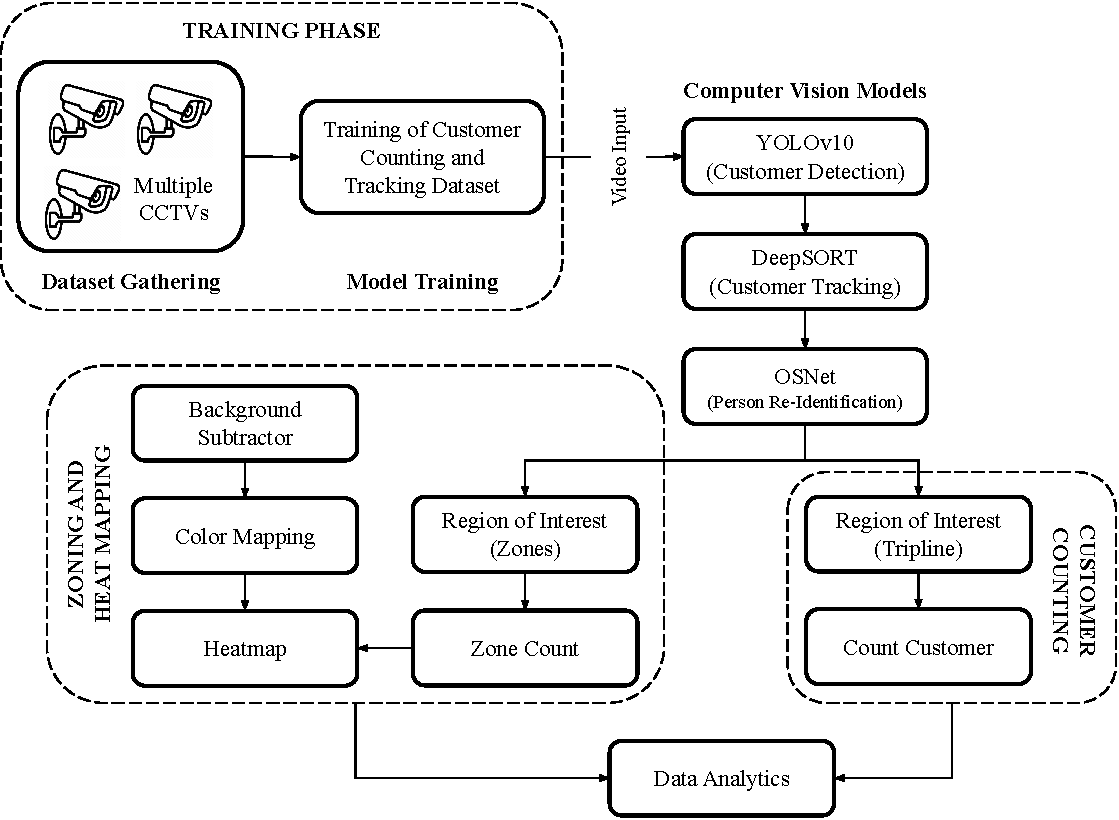
\includegraphics[width=0.85\linewidth]{fig/2.1.pdf}
	\label{fig:2.1}
\end{figure}

}